\begin{subfigure}[t]{0.45\textwidth}
\centering
\begin{subfigure}[t]{\textwidth}
    \centering
    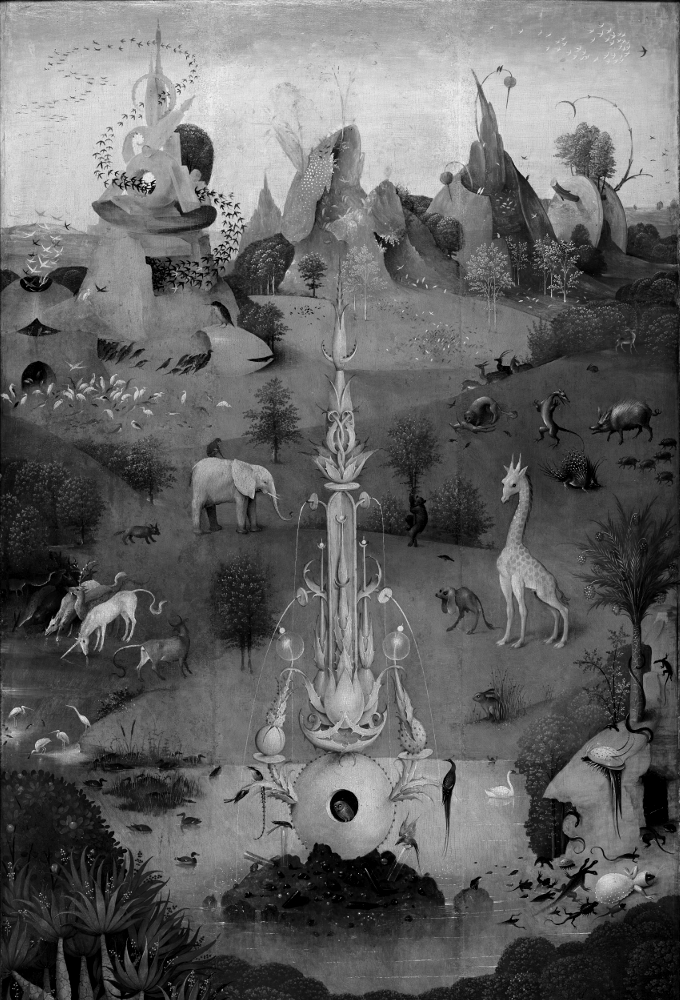
\includegraphics[width=\textwidth]{images/A1.png}
    \caption{Une première perspective marquée et s'étendant au loin. Ici, l'auditeur peut explorer une ménagerie positionnée en trois dimensions, ainsi que des sons doux émanant de la structure centrale.}
    \label{fig.a1}
\end{subfigure}~\\       
\begin{subfigure}[t]{\textwidth}
    \centering
    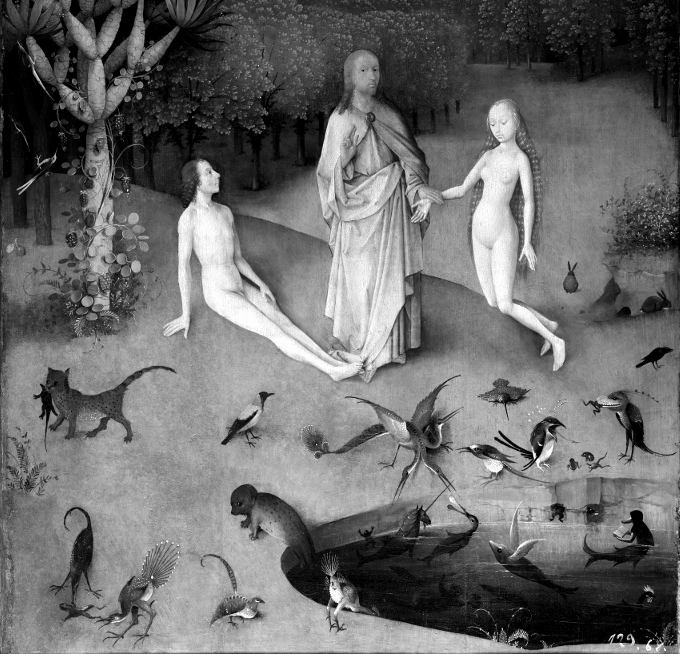
\includegraphics[width=\textwidth]{images/A2.png}
    \caption{Une scène faisant référence à la Genèse. Plusieurs scénarios sont possibles en fonction de l'ordre dans lequel les personnages sont actionnés.}
    \label{fig.a2}
\end{subfigure}   
\label{fig.a}
\end{subfigure}